\section{Background}

Generating token predictions for network configurations requires knowledge of multiple domains. In this section we introduce router configurations and the tools available for writing as well as managing them. We also expand on some code completion techniques that have been successful for programming languages, and form a basis our engine.

\subsection{Network Configurations} 

Router configuration files are often written in a vendor specific language, the popular ones being provided by Cisco and Junyper systems. These files often exist as plain text on the routers and are composed of different types of `stanzas'. A stanza is defined as the largest contiguous block of commands that encapsulate a piece of the router's functionality. The most important types of stanzas include routing protocol, access-control list (ACL), and interface. Each stanza describes the router's particular role in relation to the stanza type. Consider the configuration file for the router with hostname A in Figure 1. We can see an ACL stanza near the top which is configured to deny communication from any IP address beginning with 12. A few interface stanzas follow right below it, which define how this router is connected to other routers with some details about the connections (such as costs associated with using those routes). Lastly, at the bottom, we see a routing protocol stanza which states that the router uses the OSPF protocol to connect to two subnets.  

Network operators will configure these stanzas to define how the routers interact with each other. For example, operators might specify which devices the given router is connected to and what protocol it should follow when communicating with such devices. Additionally, they could enforce security measures by using access-control lists to block certain hosts from entering or leaving a network. 

Here we can see some inklings of general purpose programming languages. 

\begin{figure}[H]
	\centering
	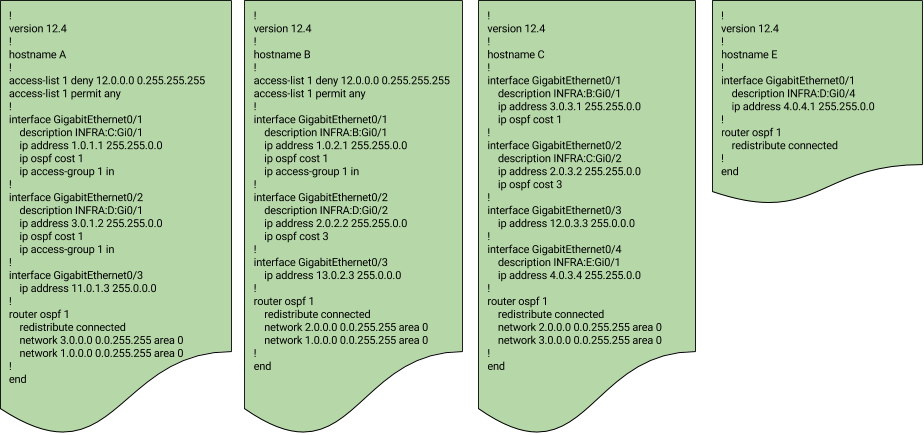
\includegraphics[width=5in]{configexample.png}
	\caption{A set of simplified configurations for a small network with four routers employing a single OSPF protocol.}
\end{figure}

\subsection{Network Management Tools}

Network management tools are built to assist network operators as they design and manage router configurations. Most of these tools offer some form a Command Line Interface, where the operators can use vendor  specific languages to update router configurations. Often, these CLIs will offer rudimentary tab completion, where they will alphabetically suggest all the options available for a token from the invocation point. These are sometimes unhelpful as the user then has to search for the desired completion.\\ 

A recurring drawback of these tools is that they focus mostly on updating existing configurations. They do not provide any additional functionality for writing new configurations other than utilizing templates. Even in the latter case, the operators will have to fill in the templates appropriately or write their own custom templates for specialized router roles. Our work acknowledges that in practice no network’s functionality can be captured by templates alone. Thus, there is a need for an engine that can distinguish itself from these existing tools by being agnostic towards where it is used in the network development life cycle. We expect our engine to perform consistently whether invoked while writing new configurations or updating existing ones.

\subsection{Code Completion}

Traditional completion techniques, such as those seen in IDEs, generate context aware models of program histories. In doing so, code completion engines often have to be aware of the grammar of the programming language and make suggestions based off that. These solutions offer fairly respectable accuracies but come with their idiosyncrasies. Popular IDEs, such as IntelliJ or Eclipse, use relatively simple type based inferential techniques to suggest all methods available for an object, usually sorted in alphabetical order. Researchers, on the other hand, have proposed more ‘intelligent’ forms of code completion techniques in the past. Early work started by adopting rule based approaches where a database of predefined rules could be continuously queried to carry out possible completion tasks~\cite{kaiser}.  Other researchers explored how to make use of program history to offer suggestions based on what users had done in the past~\cite{robbes}.\\  

Eventually people started applying machine learning techniques, such as KNNs, to extract patterns from existing code bases and building models that could be used to rank possible predictions for a given input vector. All these techniques, however, require some form of context extraction, so that information about the codebase can be stored e.g. in form of a feature vector.They heavily leverage the existing code structure and require knowledge about the grammar of the programming language. A similar methodology for network configurations would require more input from our end to ensure that the context of the tokens was properly understood. However, NLP techniques can generate predictions based on token usage and do not need to be explicitly aware of the grammar. This allows us to use these techniques independent of vendor specific configuration languages. 

\subsection{N-gram Models}

Consider a sequence of tokens in a body of text (in our case, network configurations). We can statistically model how likely tokens are to follow other tokens. We accomplish this by calculating the conditional probabilities of certain tokens appearing in the text. Given a sequence of tokens $a_1,a_2,a_3,...,a_n$, we can calculate the probability of $a_2$ occurring given that $a_1$ has already occurred i-e $p(a_2 | a_1)$. We continue by calculating the probability of $a_3$ given $a_2$, and so on. These probabilities would be estimated by counting the frequency by which a given pair occurs in our training data. Since we looked at two tokens at a time, this is called a bigram model. More generally, predicting how likely a token is to show up based on the previous $n-1$ tokens is called an n-gram model. In our work, we plan to use bigram and trigram models.

\subsection{Likelihood estimators} 

Likelihood ratios are one approach to hypothesis testing. The two hypotheses in our case are:

\begin{center}
Hypothesis 1: $P(w_2|w_1) = p = P(w_2|\neg w_1)$ \\
Hypothesis 2: $P(w_2|w_1) = p_1 \neq p_2 = P(w_2|\neg w_1)$	\\	
\end{center}

A likelihood estimator is simply a number that tells us how much more likely one hypothesis is than the other. They also have an added advantage of generally being more appropriate for sparse data than other tests. Our system internally uses the Manning and Schutze (5.3.4) version of likelihood estimators~\cite{manning}.
